\chapter{Manifols and Tensor Fiels}
In this chapter we lay the foundations for a precise, mathematical formulation of general relativity by obtaining some basic properties of manifols and tensor fiels. As defined in section 2.1, an $n$-dimensional manifold is a set that has the local differential structure of $\mathbb{R}^n$ but not necessarily its global properties. In section 2.2 we define tangent vectors as directional derivative operators acting on functions defined on a manifold. We obtain there some important properties of coordinate bases of the tangent space and tangents to curves. Tensors are introduced in section 2.3, and the notion of a metric is defined. Finally, in section 2.4 we introduce the abstract index notation for tensors, which we shall use throughout the remainder of this book. We will use a fair number of standard mathematical symbols in this chapter, and the reader unfamiliar with these symbols should consult the section ``Notation and Conventions'' at the beginning of this book.

\section{Manifols}
As mentioned in the previous chapter, our experience tells us that spacetime is a ``four-dimensional continuum'' in the sense that it requires four numbers to characterize an event. In prerelativity physics as well as in special relativity it is assumed that this is globally true, i.e., that all events in spacetime can be put into one-to-one continuous correspondence with the points of $\mathbb{R}^4$. However, in general relativity we will be solving for the spacetime geometry and we do not wish to prejudice in advance any aspects of the global nature of spacetime structure. Our situation is very similar to that of hypothetical investigators of the structure of the surface of Earth prior to the explorations of Columbus and Magellan. Such investigators might notice that in their vicinity they can characterize positions on the surface of the Earth by two numbers. However, they would be making a serious error is they were to extrapolate from this fact to the conclusion that the entire collection of points on the surface of the Earth can be put into one-to-one correspondence with points of $\mathbb{R}^2$ in a continuous manner. Thus, what is needed as a mathematical basis for beginning the investigation of spacetime structure (as well as the surface of the Earth) is a precise notion of a manifold, that is, a set in which the vicinity of every point ``looks like'' $\mathbb{R}^n$ but which may have quite different global properties.

In the case of the Earth, our investigators might be aware that its surface ``lives'' in the higher dimensional Euclidean space $\mathbb{R}^3$ of all space points (at least, according to prerelativity notions of space and time). Thus the study of two-dimensional surfaces embedded in  $\mathbb{R}^3$ would provide an adequate mathematical framework to analyze the structure of the Earth's surface, and one could avoid making an abstract definition of manifols. However, in general relativity, spacetime itself does not (as far as we know) naturally live in a higher dimensional Euclidean space, so an abstract definition is much more natural. Indeed, such a definition turns out to be extremely useful even for the study of ordinary surfaces in $\mathbb{R}^3$.

Before defining the notion of a manifold we remind the reader that an \emph{open ball} in $\mathbb{R}^n$ of radius $r$ centered around point $y=(y^1,\ldots,y^n)$ consists of the points $x$ such that $\abs{x-y}<r$, where

\[\textstyle\abs{x-y}=\ab[\sum_{\mu=1}^n(x^\mu-y^\mu)^2]^{1/2}\]

An \emph{open set} in $\mathbb{R}^n$ is any set which can be expressed as a union of open balls. This notion of open set makes $\mathbb{R}^n$ a topological space in the sense discussed in appendix A.

Basically, a \emph{manifold} is a set made up of pieces that ``look like'' open subsets of $\mathbb{R}^n$ such that these pieces can be ``sewn together'' smoothly. More precisely, an \emph{$n$-dimensional}, $C^\infty$, \emph{real manifold $M$} is a set together with a collection of subsets $\{O_\alpha\}$ satisfying the following properties
\begin{enumerate}[label=(\arabic*)]
    \item Each $p\in M$ lies in at least one $O_\alpha$, i.e., the $\{O_\alpha\}$ cover $M$.
    \item For each $\alpha$, there is a one-to-one, onto, map $\psi_\alpha:\ O_\alpha\to U_\alpha$, where $U_\alpha$ is an open subset of $\mathbb{R}^n$.
    \item If any two sets $O_\alpha$ and $O_\beta$ overlap, $O_\alpha\cap O_\beta\neq\varnothing$ (where $\varnothing$ denotes the empty set), we can consider the map $\psi_\beta\circ\psi_\alpha^{-1}$ (where $\circ$ denotes composition) which takes points in $\psi_\alpha[O_\alpha\cap O_\beta]\subset U_\alpha\subset\mathbb{R}^n$ to points in $\psi_\beta[O_\alpha\cap O_\beta]\subset U_\beta\subset\mathbb{R}^n$ (see \figref{2.1}). We require these subsets of $\mathbb{R}^n$ to be open and this map to be $C^\infty$, i.e., infinitely continuously differentiable. (Since we are dealing here with maps of $\mathbb{R}^n$ into $\mathbb{R}^n$, the advanced calculus notion of $C^\infty$ functions applies.)
\end{enumerate}

Each map $\psi_\alpha$ is generally called a \emph{chart} by mathematicians and a \emph{coordinate system} by physicists. We shall use these terms interchangeably. In order to prevent one from defining new manifolds by merely deleting or adding in a coordinate system, it is convenient also to require in the definition of $M$ that the cover $\{O_\alpha\}$ and chart family $\{\psi_\alpha\}$ is maximal, i.e., all coordinate systems compatible with (2) and (3) are included. The definition of $C^k$ or analytic manifolds is the same as above with the appropriate change in requirement (3). To define a complex manifold, one merely replaces $\mathbb{R}^n$ by $\mathbb{C}^n$ above.

\begin{figure}[!ht]
    \centering
    \begin{tikzpicture}
        \node [inner sep=0pt] at (0,0) {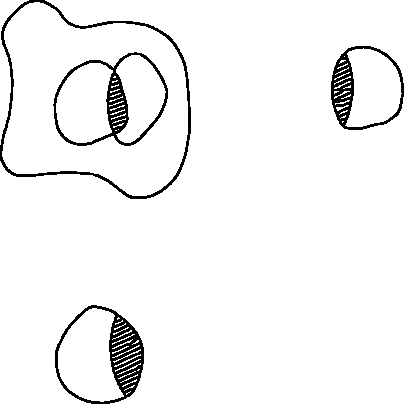
\includegraphics{fig2.1}};
        \node at (-2.75,2.75) {$\scriptstyle\mathsf{M}$};
        \node at (-2,1.75) {$\scriptstyle O_\alpha$};
        \node at (-1,1.75) {$\scriptstyle O_\beta$};
        \draw (-2.875,-1.25) rectangle (-.625,-3.75) node [at start, below right] {$\scriptstyle\mathsf{R}^n$};
        \draw (1.5,3) rectangle (3.75,.75) node [at start, below right] {$\scriptstyle\mathsf{R}^n$};
        \draw [->] (-2,1.5) -- (-2,-2.5) node [midway,right] {$\scriptstyle\psi_\alpha$} node [below] {$\scriptstyle U_\alpha$};
        \draw [->] (-.8,1.9) -- (2.8,1.9) node [midway,above] {$\scriptstyle\psi_\beta$} node [right] {$\scriptstyle U_\beta$};
        \draw [->] (-1.25,-2.5) -- (2.5,1.75) node [midway,above,sloped] {$\scriptstyle\psi_\beta\circ\psi_\alpha^{-1}$};
    \end{tikzpicture}
    \caption{An illustration of the map $\psi_\beta\circ\psi_\alpha^{-1}$ arising when two coordinate systems overlap.}
    \label{2.1}
\end{figure}
 
We can define a topology on the manifold $M$ by demanding that all the maps $\psi_\alpha$ in our maximal collection be homeomorphisms (see appendix A for definitions). Indeed, it is perhaps more natural to proceed by defining a manifold to be a topological space satisfying the above properties, with each $\psi_\alpha$ a homeomorphism. (We have not done so simply in order to avoid introducing the machinery of topological spaces in the main text.) Viewed as topological spaces, we shall consider in this book only manifolds which are \emph{Hausdorff} and \emph{paracompact}; these terms are explained in appendix A.

Euclidean space $\mathbb{R}^n$ provides a trivial example of a manifold, which can be covered by a single chart ($O=\mathbb{R}^n$, $\psi=\text{identity map}$). A more interesting example of a manifold is the $2$-sphere $S^2$
 \[S^2=\ab\{\ab(x^1,x^2,x^3)\in\mathbb{R}|\ab(x^2)^2+\ab(x^2)^2+\ab(x^3)^2=1\}\]

The entire $2-$sphere $S^2$ cannot be mapped into $\mathbb{R}^2$ in a continuous, $1-1$ manner, but ``pieces'' of $S^2$ can, and these can be ``smoothly sewn together''. For example, if we define the six hemispherical open sets $O_i^\pm$ for $i=1,2,3$ by
\[
    O_i^\pm=\ab\{\ab(x^1,x^2,x^3)\in S^2|\pm x^i>0\}
\]

then $\ab\{O_i^\pm\}$ covers $S^2$. Furthermore, each $O_i^\pm$ can be mapped homeomorphically into the open disk $D=\ab\{(x,y)\in\mathbb{R}^2|x^2+y^2<1\}$ in the plane via the ``projection maps'' $f_1^+:O_1^+\to D$, $f_1^-:O_1^-\to D$, etc., defined by $f_1^+(x^1,x^2,x^3)=(x^2,x^3)$, etc. The overlap functions $f_i^\pm\circ(f_j^\pm)^{-1}$ can be checked to be $C^\infty$ in their domain of definition (problem 1). Thus, $S^2$ is a two-dimensional manifold. In a similar manner, the $n$-dimensional sphere $S^n$ is seen to be a manifold.

Given two manifolds $M$ and $M'$ of dimension $n$ and $n'$, respectively, we can make the product space $M\times M'$ consisting of all pairs $(p,p')$ with $p\in M$ and $p'\in M'$ into an $(n+n')$-dimensional manifold as follows. If $\psi_\alpha:O_\alpha\to U_\alpha$ and $\psi_\beta':O_\beta'\to U_\beta'$ are charts, we define a chart $\psi_{\alpha\beta}:O_{\alpha\beta}\to U_{\alpha\beta}\subset\mathbb{R}^{n+n'}$ on $M\times M'$ by taking $O_{\alpha\beta}=O_\alpha\times O_\beta'$, $U_{\alpha\beta}=U_\alpha\times U_\beta'$, and setting $\psi_{\alpha\beta}(p,p')=[\psi_\alpha(p),\psi_\beta'(p')]$. it is easily checked that the chart family $\{\psi_{\alpha\beta}\}$ satisfies the properties required to define a manifold structure on $M\times M'$. Most manifolds we will consider in this book can be expressed as products of Euclidean space $\mathbb{R}^n$ with spheres $S^m$.

With the structure on manifolds given by the coordinate systems, we may now define the notion of differentiability and smoothness of maps between manifolds. Let $M$ and $M'$ be manifolds and let $\{\psi_\alpha\}$ and $\{\psi_\beta'\}$ denote the chart maps. A map $f:M\to M'$ is said to be $C^\infty$ if for each $\alpha$ and $\beta$, the map $\psi_\beta'\circ f\circ\psi_\alpha^{-1}$ taking $U_\alpha\subset\mathbb{R}^n$ into $U_\beta'\subset\mathbb{R}^n$ is $C^\infty$ inverse, $f$ is called a \emph{diffeomorphism} and $M$ and $M'$ are said to be \emph{diffeomorphic}. Diffeomorphic manifolds have identical manifold structure.

\section{Vectors}
The concept of a vector space is undoubtedly familiar to most readers. In prerelativity physics it is assumed that space has the natural structure of a three-dimensional vector space once one has designated a point to serve as the origin; the natural rules for adding and scalar multiplying spatial displacements satisfy the vector space axioms\footnote{See, e.g., Royden (1963) for the list of vector space axioms.}. In special relativity, spacetime similarly has the natural structure of a four-dimensional vector space. However, when one considers curved geometries (as we do in general relativity), this vector space structure is lost. For example, there is no natural notion of how to ``add'' two points on a sphere and end up with a third point on the sphere. Nevertheless, vector space structure can be recovered in the limit of ``infinitesimal displacements'' about a point. It is this notion of ``infinitesimal displacements'' or tangent vectors which lies at the foundation of calculus on manifolds. Therefore, we will devote considerable attention below to giving a precise mathematical definition of this concept.

For manifolds like the sphere, which arise naturally as surfaces embedded in $\mathbb{R}^n$ the intuitive notion of a tangent vector at point $p$ is a vector lying in the tangent plane illustrated in \figref{2.2}. For manifolds embedded in $\mathbb{R}^n$, this idea can be made mathematically precise. However, in many situations-most importantly in general relativity-one is given a manifold without an embedding of it in $\mathbb{R}^n$. Thus, it is important (and, in the long run, much more useful) to define a tangent vector in a way that refers only to the intrinsic structure of the manifold, not to its possible embeddings in $\mathbb{R}^n$.

\begin{figure}[!ht]
\centering
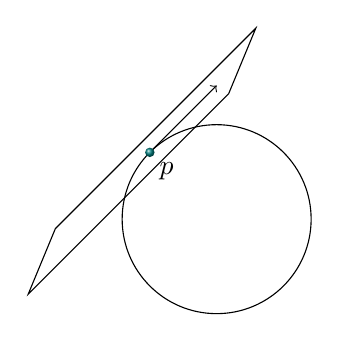
\begin{tikzpicture}
    \draw (0,0) circle (1.2);
    \draw [->] ({-1.2/sqrt(2)},{1.2/sqrt(2)}) --++ ({1.2/sqrt(2)},{1.2/sqrt(2)}) node [at start,below right] {$p$};
    \shade [ball color=teal] ({-1.2/sqrt(2)},{1.2/sqrt(2)}) circle (.06);
    \draw [xshift=(-1.2/sqrt(2)-1.2)*1cm,yshift=(-1.2/sqrt(2)+0.9-0.45*cos(22.5)+0.45*sin(22.5)/sin(45))*1cm] (0,0) -- ({1.8*sqrt(2)},{1.8*sqrt(2)}) --++ ({-.9*sin(22.5)},{-.9*cos(22.5)}) --++ ({-1.8*sqrt(2)},{-1.8*sqrt(2)}) -- cycle;
\end{tikzpicture}
\caption{The tangent plane at point $p$ of a sphere in $\mathbb{R}^3$.}
\label{2.2}
\end{figure}

Such a definition is provided by the notion of a tangent vector as a directional derivative. In $\mathbb{R}^n$ there is a one-to-one correspondence between vectors and directional derivatives. A vector $v=(v^1,\ldots,v^n)$ defines the directional derivative operator $\sum_\mu v^\mu(\partial/\partial x^\mu)$ and vice versa. Directional derivatives are characterized by their linearity and ``Leibnitz rule'' behavior when acting on functions. Thus on a manifold $M$ let $\mathscr{F}$ denote the collection of $C^\infty$ functions from $M$ into $\mathbb{R}$. We define a tangent vector $v$ at point $p\in M$ to be a map $v:\mathscr{F}\to\mathbb{R}$ which (1) is linear and (2) obeys the Leibnitz rule
\begin{enumerate}[label=(\arabic*)]
    \item $v(af+bg)=av(f)+bv(g)$, for all $f$, $g\in\mathscr{F}$; $a$, $b\in\mathbb{R}$.
    \item $v(fg)=f(p)v(g)+g(p)v(f)$.
\end{enumerate}

Note that (1) and (2) imply that if $h\in\mathscr{F}$ is a constant function. i.e., $h(q)=c$ for all $q\in M$, then $v(h)=0$, since from (2) we have $vv{v}(h^2)=2cv(h)$ whereas from (1) we have $v(h^2)=v(ch)=cv(h)$.

Though it may not be obvious at first glance, this definition does indeed make precise and give intrinsic meaning to the concept of an ``infinitesimal displacement''. In the first place, it is easy to see that the collection, $V_p$, of tangent vectors at $p$ has the structure of a vector space under the addition law $(v_1+v_2)(f)=v_1(f)+v_2(f)$ and scalar multiplication law $(av)(f)=av(f)$. A second vital property of $V_p$, is given by the following theorem

\begin{theorem}
    \itshape Let $M$ be an $n$-dimensional manifold. Let $p\in M$ and let $V_p$ denote the tangent space at $p$. Then $\dim V_p=n$.
\end{theorem}
\begin{figure}[!ht]
\centering
\begin{tikzpicture}
    \node at (0,0) {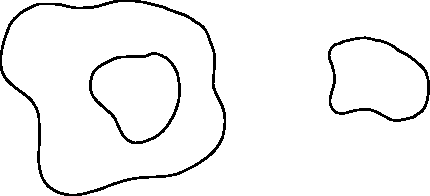
\includegraphics{fig2.3.pdf}};
    \draw [semithick] (1.25,1.75) rectangle (3.75,-1.25) node [at start,below right] {$\scriptstyle\mathsf{R}^n$};
    \draw [<->,semithick] (1.75,-.25) -- (1.75,-.75) node [at start,left,xshift=.25em] {$\scriptstyle x^2$} -- (2.25,-.75) node [below,yshift=.25em] {$\scriptstyle x^1$};
    \draw [->,semithick] (-.75,.25) -- (2.5,.25) node [above] {$\scriptstyle U$} node [midway,above] {$\scriptstyle\psi$};
    \shade [ball color=teal] (-1,.25) circle (.06) node [left] {$\scriptstyle p$};
    \shade [ball color=teal] (2.5,.125) circle (.06) node [right] {$\scriptstyle\psi(p)$};
    \draw [->,semithick] (-1,-.25) -- (-1,-4) node [at start,left] {$\scriptstyle O$} node [midway,right] {$\scriptstyle f$};
    \draw [semithick] (-4,-4) -- (0,-4) node [above left] {$\scriptstyle\mathsf{R}$};
\end{tikzpicture}
\caption{A diagram illustrating the definition of the directional derivatives $X_\mu$, used in theorem 2.2.1.}
    \label{2.3}
\end{figure}
\begin{proof}
    We shall show that $\dim V_p=n$ by constructing a basis of $V_p$, i.e., by finding $n$ linearly independent tangent vectors which span $V_p$. Let $\psi:O\to U\subset\mathbb{R}^n$ be a chart with $p\in O$ (see \figref{2.3}). If $f\in\mathscr{F}$, then by definition $f\circ\psi^{-1}:U\to\mathbb{R}$ is $C^\infty$. For $\mu=1,\ldots,n$ define $X_\mu:\mathscr{F}\to\mathbb{R}$ by
\begin{equation}
    X_\mu(f)=\pdv{}{X^\mu}(f\circ\psi^{-1})\bigg|_{\psi(p)}
\end{equation}

where $(x^1,\ldots,x^n)$ are the Cartesian coordinates of $\mathbb{R}^n$. Then $X_1,\ldots,X_n$ are tangent vectors, and it is easily seen that they are linearly independent. To show that they span $V_p$ we make use of the following result from advanced calculus (see problem 2): If $F:\mathbb{R}^n\to\mathbb{R}$ is $C^\infty$, then for each $a=(a^1,\ldots,a^n)\in\mathbb{R}^n$ there exists $C^\infty$ functions $H_\mu$ such that for all $x\in\mathbb{R}^n$ we have
\begin{equation}
    F(x)=F(a)+\sum_{\mu=1}^n(x^\mu-a^\mu)H_\mu(x)
    \label{2.2.2}
\end{equation}

Furthermore, we have
\begin{equation}
    H_\mu(a)=\pdv{F}{x^\mu}\bigg|_{x=a}
    \label{2.2.3}
\end{equation}

We apply this result here, letting $F=f\circ\psi^{-1}$ and $a=\psi(p)$. Then, for all $q\in O$ we have
\begin{equation}
    f(q)=f(p)+\sum_{\mu=1}^n\ab[x^\mu\circ\psi(q)-x^\mu\circ\psi(p)]H_\mu(\psi(q))
    \label{2.2.4}
\end{equation}

Let $v\in V_p$. We wish to show that $v$ is a linear combination of $X_1,\ldots,X_n$. To do so, we apply $v$ to $f$, using \eqref{2.2.4}, the linearity and Leibnitz properties of $v$, and the fact that $v$ applied to a constant [such as $f(p)$] vanished. We obtain
\begin{equation}
\begin{aligned}
    f(q)= & f(p)+\sum_{\mu=1}^n\Bigg\{\ab[x^\mu\circ\psi(q)-x^\mu\circ\psi(p)]\bigg|_{q=p}v(H_\mu\circ\psi)\\
    & +(H_\mu\circ\psi)\bigg|_pv\ab[x^\mu\circ\psi-x^\mu\circ\psi(p)]\Bigg\}\\
    = & \sum_{\mu=1}^n[H_\mu\circ\psi(p)]v(x^\mu\circ\psi)
\end{aligned}
\label{2.2.5}
\end{equation}

But by \eqref{2.2.3}, $H_\mu\circ\psi(p)$ is just $X_\mu(f)$. Thus, for all $f\in\mathscr{F}$, we have
\begin{equation}
    \vv{f}=\sum_{\mu=1}^nv^\mu X_\mu(f)
    \label{2.2.6}
\end{equation}

where the coefficients $v^\mu$ are the values of $v$ applied to the function $x^\mu\circ\psi$
\begin{equation}
    v^\mu=v(x^\mu\circ\psi)
    \label{2.2.7}
\end{equation}

Thus, we have expressed an arbitrary tangent vector $v$ as a sum of the $X_\mu$
\begin{equation}
    v=\sum_{\mu=1}^nv^\mu X_\mu
    \label{2.2.8}
\end{equation}

which completes the proof.
\end{proof}

The basis $\{X_\mu\}$ of $V$, introduced in the proof of theorem 2.2. 1 is called a \emph{coordinate basis} and is of considerable importance in its own right. Frequently, one denotes $X_\mu$ as simply $\partial/\partial x^\mu$. Had we chosen a different chart, $\psi'$, we would have obtained a different coordinate basis $\{X_\nu'\}$. We can, of course, express $X_\mu$ in terms of the new basis $\{X_\nu'\}$. Using the chain rule of advanced calculus, we have
\begin{equation}
    X_\mu=\sum_{\nu=1}^n\pdv{x'^\nu}{x^\mu}\bigg|_{\psi(p)}X_\nu'
    \label{2.2.9}
\end{equation}

where $x'^\nu$ denotes the $\nu$th component of the map $\psi'\circ\psi^{-1}$. Hence, from \eqref{2.2.8} and \eqref{2.2.9} we find that the components $v'^\nu$ of a vector $v$ in the new coordinate basis are related to the components $v^\mu$ in the old basis by
\begin{equation}
    v'^\nu=\sum_{\mu=1}^nv'^\mu\pdv{x'^\nu}{x^\mu}
    \label{2.2.10}
\end{equation}

\Eqref{2.2.10} is known as the \emph{vector transformation law}.

A \emph{smooth curve}, $C$, on a manifold $M$ is simply a $C^\infty$ map of $\mathbb{R}$ (or an interval of $\mathbb{R}$) into $M$, $C:R \to M$. At each point $p\in M$ lying on the curve $C$ we can associate with $C$ a tangent vector $T\in V_p$, as follows. For $f\in\mathscr{F}$ we set $T(f)$ equal to the derivative of the function $f\circ C:\mathbb{R}\to\mathbb{R}$ evaluated at $p$, i.e., $T(f)=\d(f\circ C)/\d t$. Note that the above coordinate basis vector $X_\mu$, associated with a chart $\psi$ is the tangent to the curves on $M$ obtained by keeping all coordinate values except $x^\mu$ constant. Notice also that when we choose a coordinate system $\psi$, the curve $C$ on $M$ will get mapped into a curve $x^\mu(t)$ in $\mathbb{R}^n$. Then, for any $f\in\mathscr{F}$, we have
\begin{equation}
    T(f)=\odv{}t(f\circ C)=\sum_\mu\pdv{}{x^\mu}(f\circ\psi^{-1})\odv{x^\mu}t=\sum_\mu\odv{x^\mu}tX_\mu(f)
    \label{2.2.11}
\end{equation}

Thus, in any coordinate basis, the components $T^\mu$ of the tangent vector to the curve are given by
\begin{equation}
    T^\mu=\odv{x^\mu}t
    \label{2.2.12}
\end{equation}

In the discussion above, we fixed a point $p\in M$ and considered the tangent space, $V_p$, at $p$. At another point $q\in M$ we could, of course, define $V_q$. It is important to emphasize that, given only the structure of a manifold, there is no natural way of identifying $V_q$ with $V_p$; that is, there is no way of determining whether a tangent vector at $q$ is ``the same'' as a tangent vector at $p$. In chapter 3, we shall see that when additional structure is given (namely, a connection or derivative operator on the manifold), one has a notion of ``parallel transport'' of vectors from $p$ to $q$ along a curve joining these points. However, if the curvature is nonzero, the identification of $V_p$ with $V_q$ obtained in this manner will depend on the choice of curve.

A \emph{tangent field}, $v$, on a manifold $M$ is an assignment of a tangent vector, $v|_p\in V_p$, at each point $p\in M$. Despite the fact that the tangent spaces $V_p$ and $V_q$ at different points are different vector spaces, there is a natural notion of what it means for o to vary smoothly from point to point. If f is a smooth ($C^\infty$) function, then at each $p\in M$, $v|_p(f)$ is a number, i.e., $v(f)$ is a function on $M$. The tangent field o is said to be \emph{smooth} if for each smooth function $f$, the function $v(f)$ is also smooth. Since the coordinate basis fields $X_\mu$ are easily verified to be smooth, it follows that a vector field $v$ is smooth if and only if its coordinate basis components, $v^\mu$, are smooth functions.

In the heuristic discussion above, we described tangent vectors as ``infinitesimal displacements''. We shall now show that precise meaning can be given to this idea. Let $M$ be a manifold. A \emph{one-parameter group of diffeomorphisms} $\psi_t$ is a $C^\infty$ map from $\mathbb{R}\times M\to M$ such that for fixed $t\in\mathbb{R}$, $\phi_t:M\to M$ is a diffeomorphism and for all $t,s\in R$, we have $\phi_t\circ\phi_s=\phi_{t+s}$ (In particular, this last relation implies that $\phi_{t=0}$ is the identity map). We can associate to d, a vector field o as follows: for fixed $p\in M$, $\phi_t(p):\mathbb{R}\to M$ is a curve, called an \emph{orbit} of $\phi_t$, which passes through $p$ at $t=0$. Define $v|_p$ to be the tangent to this curve at $t=0$. Thus, associated to a one-parameter group of (finite) transformations of $M$ is a vector field, $v$, which can be thought of as the infinitesimal generator of these transformations.

Conversely, given a smooth vector field, $v$, on $M$ we can ask if it is possible to find \emph{integral curves} of $v$, that is, a family of curves in $M$ having the property that one and only one curve passes through each point $p\in M$ and the tangent to this curve at $p$ is $v|_p$. The answer is yes: If we pick a coordinate system in a neighborhood of $p$ as in the proof of theorem 2.2.1, we see that the problem of finding such curves reduces to solving the system
\begin{equation}
    \odv{x^\mu}t=v^\mu(x^1,\ldots,x^n)
    \label{2.2.13}
\end{equation}

of ordinary differential equations in $\mathbb{R}^n$, where $v^\mu$ is the $\mu$th component of $v$ in the coordinate basis $\{\partial/\partial x^\mu\}$. Such a system of equations has a unique solution given a starting point at $t=0$, and thus every smooth vector field $v$ has a unique family of integral curves (see, e.g., Coddington and Levinson 1955). Given the integral curves, for each $p\in M$ we define $\phi_t(p)$ to be the point lying at parameter $t$ along the integral curve of $v$ starting at $p$. Except for potential problems arising from the possibility that the integral curves of $v$ may extend to only a finite value of the curve parameter, $\phi_t$, will be a one-parameter group of diffeomorphisms.

Finally, we note that given two smooth vector fields $v$ and $w$ it is possible to define a new vector field, $[v,w]$, called the \emph{commutator} of $v$ and $w$, by
\begin{equation}
    [v,w](f)=v[w(f)]-w[v(f)]
    \label{2.2.14}
\end{equation}

(see problem 3). We note that the commutator of any two vector fields $X_\mu$ and $X_\nu$ occurring in a coordinate basis vanishes. (This fact follows directly from the definition of the coordinate basis given in the proof of theorem 2.2.1 together with the equality of mixed partial derivatives in $\mathbb{R}^n$.) Conversely, given a collection $X_1,\ldots,X_n$, of nonvanishing vector fields which commute with each other and are linearly independent at each point, one can always find a chart for which they are the coordinate basis vector fields (see problem 5). 

\section{Tensors; the Metric Tensor}
Given the notion of displacement vectors, the notion of tensors arises when one considers other quantities of interest. It turns out that many quantities have a linear (or multilinear) dependence on displacements. Consider, for example, a measurement of the magnetic field (say, in the context of prerelativity physics). For each probe orientation, a number is recorded: the magnetic field strength in that given direction. Since there is an infinite number of possible orientations of the probe, in principle an infinite number of readings would be needed to determine the magnetic field. However, this is not necessary because the magnetic field strength has a linear dependence on the probe orientation. All that is required is readings in three linearly independent probe directions; the reading in any other probe direction is equal to a linear combination of these readings.

This fact gives rise to the notion of the magnetic field as a vector or, more precisely, a dual vector. One could define a dual vector as a collection of three numbers (i.e., the probe readings) associated with a basis of spatial displacement vectors (the three independent probe directions) which transform in an appropriate manner when the basis is changed. However, we will give below a simpler and more direct definition of a dual vector as a linear map from spatial displacement vectors into numbers. We have defined the magnetic field as a dual vector here, but, as we shall see at the end of this section, because space has a metric defined on it, we can naturally associate to any dual vector an ordinary (spatial displacement) vector.

In a similar manner, other quantities that occur in physics have a similar linear dependence on spatial displacement vectors but may be functions of more than one such vector. For example, for an ordinary material body in equilibrium, consider the plane with normal vector $\vv{n}$ passing through a point $p$ in the body. At $p$, one could measure the force per unit area, $F$, in the $\vv{l}$-direction exerted on the matter on one side of the plane by the matter on the other side. One finds that $F$ depends linearly on the choice of $\vv{n}$ and $\vv{l}$. Thus, although there is an infinite number of possible choices of $\vv{n}$ and $\vv{l}$, the value of $F$ for any $\vv{n}$ and $\vv{l}$ can be calculated by knowing $3\times 3$ numbers, namely the values $F$ takes when $\vv{n}$ and $\vv{l}$ point in basis directions. This motivates the definition of a tensor which will be given below: A tensor is a multilinear (i.e., linear in each variable) map from vectors (or dual vectors) into numbers. The tensor which maps the pair of vectors $(\vv{n}, \vv{T})$ into the value of $F$ is known as \emph{the stress tensor} of the material body at $p$.

We give now the precise mathematical definition of tensors and discuss their properties. Let $V$ be any finite-dimensional vector space over the real numbers. (The case of prime interest for us is the tangent space, $V=V_p$.) Consider the collection, $V^*$, of linear maps $f:V\to\mathbb{R}$. If one defines addition and scalar multiplication of such linear maps in the obvious way, one gets a natural vector space structure on $V^*$. We call $V^*$ \emph{the dual vector space} to $V$, and elements of $V^*$ are called \emph{dual vectors}. If $v_1,\ldots,v_n$ is a basis of $V$, we can define elements $v^{1^*},\ldots,v^{n^*}$ by
\begin{equation}
    v^{\mu^*}(v_\nu)={\delta^\mu}_\nu
    \label{2.3.1}
\end{equation}

Where ${\delta^\mu}_\nu=1$ if $\mu=\nu$ and $0$ otherwise. (This defines the action of $v^{\mu^*}$ on the basis elements; its action on an arbitrary vector $v\in V$ is determined by this and linearity). It follows directly (problem 6) that $\{v^{\mu^*}\}$ is a basis of $V^*$, called the \emph{dual basis} to the basis ${v_\mu}$ of $V$. In particular, this shows that $\dim V^* = \dim V$. The correspondence $v_\mu\leftrightarrow v^{\mu^*}$ gives rise to an isomorphism between $V$ and $V^*$, but this isomorphism depends on the choice of basis $\{v_\mu\}$, so there is no natural way of identifying $V^*$ with $V$ (unless more structure is given on $V$, such as a preferred basis or, as described below, a metric).

We now can apply the above construction starting with the vector space $V^*$ thereby obtaining the \emph{double dual} vector space to $V$, denoted $V^{**}$. A vector $v^{**}$ in $V^{**}$ is a linear map from $V^*$ into $\mathbb{R}$. However, $V^{**}$ is naturally isomorphic to the original vector space $V$. To each vector $v$ in $V$ we can associate the map in $V^{**}$ whose value on the vector $\omega^*\in V^*$ is just $\omega^*(v)$. In this way, we obtain a one-to-one linear map of $V$ into $V^{**}$ which must be onto since $\dim V = \dim V^{**}$. Thus, taking the double dual gives nothing new; we can naturally identify $V^{**}$ with the original vector space $V$. This identification will be assumed in the discussion below.

We now are ready to define the notion of a tensor. Let $V$ be a finite dimensional vector space and let $V^*$ denote its dual vector space. A \emph{tensor, $T$, of type $(k,l)$} over $V$ is a multilinear map

\[T:\underset{k}{\underbrace{V^*\times\cdots\times V^*}}\times\underset{l}{\underbrace{V\times\cdots\times V}}\to\mathbb{R}\]

In other words, given $k$ dual vectors and $l$ ordinary vectors, $T$ produces a number, and it does so in such a manner that if we fix all but one of the vectors or dual vectors, it is a linear map on the remaining variable.

Thus, according to the above definition, a tensor of type $(0,1)$ is precisely a dual vector. Similarly, a tensor of type (1, 0) is an element of $V^{**}$. However, since we identify $V^{**}$ with $V$, a tensor of type $(1, 0)$ is nothing more than an ordinary vector. Because of the identification of $V^{**}$ with $V$, we may view tensors of higher type in many different (though, or course, equivalent) ways. For example, a tensor $T$ of type $(1,1)$ is a multilinear map from $V^*\times V\to\mathbb{R}$. Hence, if we fix $v\in V$, $T(\cdot,v)$ is an element of $V^{**}$, which we identify with an element of V. Thus, given a vector in $V$, $T$ produces another vector in $V$ in a linear fashion. In other words, we can view a tensor of type $(1, 1)$, as a linear map from $V$ into $V$, and vice versa. Similarly, we can view $T$ as a linear map from $V^*$ into $V^*$.

With the obvious rules for adding and scalar multiplying maps, the collection $\mathscr{T}(k, l)$ of all tensors of type $(k,l)$ has the structure of a vector space. Because of the multilinearity property, a tensor is uniquely specified by giving its values on vectors in a basis $\{v^{\nu^*}\}$ of $V$ and its dual basis $\{v^{\nu^*}\}$ of $V^*$. Since there are $n^{k+1}$ independent ways of filling the slots of a tensor of type $(k,l)$ with such basis vectors (where $n = \dim V = \dim V^*$), the dimension of the vector space $\mathscr{T}(k,l)$ is $n^{k+1}$.

We now introduce two simple but important operations on tensors, which will be used commonly in what follows. The first is called \emph{contractio}n with respect to the $i$th (dual vector) and $j$th (vector) slots and is a map $C:\mathscr{T}(k,l)\to\mathscr{T}(k-1,l-1)$ defined as follows. If $T$ is a tensor of type $(k,l)$, then

\begin{equation}
    CT=\sum_{\sigma=1}^nT(\ldots,v^{\sigma^*},\ldots;\ldots,v_\sigma,\ldots)
    \label{2.3.2}
\end{equation}

where $\{v_\sigma\}$ is a basis of $V$, $\{v^{\sigma^*}\}$ is its dual basis, and these vectors are inserted into the $i$th and $j$th slots of $T$. [Note that the contraction of a tensor of type $(1, 1)$, viewed as a linear map from $V$ into $V$, is just the trace of the map.] The tensor $CT$ thus obtained is independent of the choice of basis ${v_\mu}$, so the operation of contraction is indeed well defined (see problem 6).

The second operation on tensors is the outer product. Given a tensor $T$ of type $(k, l)$ and another tensor $T'$ of type $(k', l')$, we can construct a new tensor of type $(k+k', I+l')$ called the \emph{outer product} of $T$ and $T'$ and denoted $T\otimes T'$, by the following simple rule. Given $(k+k')$ dual vectors $v^{1^*},\ldots,v^{k+k'^*}$ and $(l+l')$ vectors $w_1,\ldots,w_{l+l'}$, we define $T\otimes T'$ acting on these vectors to be the product of $w_1,\ldots,w_{l+l'}$, and $T'\ab(v^{k+1^*},\ldots,v^{k+k'^*};w_{l+1},\ldots,w_{l+l'})$.

Thus, one way of constructing tensors is to take outer products of vectors and dual vectors. A tensor which can be expressed as such an outer product is called \emph{simple}\footnote{In many references, a tensor of type $(0,l)$ which can be expressed as the totally antisymmetric part of a simple tensor (see \eqref{2.4.4} below) also is referred to as simple.}. If $\{v_\mu\}$ is a basis of $V$ and $\ab\{v^{\nu^*}\}$ is its dual basis, it is easy to show that the $n^{k+1}$ simple tensors $\Big\{v_{\mu_1}\otimes\cdots\otimes v_{\mu_k}\otimes v^{\nu_1^*}\otimes\cdots\otimes v^{\nu_l^*}\Big\}$ yield a basis of $\mathscr{T}(k,l)$. Thus, every tensor $T$ of type $(k, l)$ can be expressed as a sum of simple tensors in this collection

\begin{equation}
    T=\sum_{\mu_1,\ldots,\nu_l=1}^n{T^{\mu_1\cdots\mu_k}}_{\nu_1\cdots\nu_l}v_{\mu_1}\otimes\cdots\otimes v^{\nu_l^*}
    \label{2.3.3}
\end{equation}

The basis expansion coefficients, ${T^{\mu_1\cdots\mu_k}}_{\nu_1\cdots\nu_l}$, are called the \emph{components} of the tensor T with respect to the basis $\{v_\mu\}$. Note that we follow the standard convention in the notation for components of using superscripts for labels $\mu_i$ associated with vectors and subscripts for labels $\nu_j$ associated with dual vectors.

In terms of components, we have the following formulas for contraction and outer product. Suppose the tensor $T$ has components ${T^{\mu_1\cdots\mu_k}}_{\nu_1\cdots\nu_l}$ as in \eqref{2.3.3}. Then, the contraction, $CT$, of $T$ has components given by
\begin{equation}
    {(CT)^{\mu_1\cdots\mu_{k-1}}}_{\nu_l\cdots\nu_{l-1}}=\sum_{\sigma=1}^n{T^{\mu_1\cdots\sigma\cdots\mu_{k-1}}}_{\nu_1\cdots\sigma\cdots\nu_{l-1}}
    \label{2.3.4}
\end{equation}

If $T'$ has components ${T'^{\mu_1'\cdots\mu_{k'}'}}_{\nu_1'\cdots\nu_{l'}'}$, then the outer product $S=T\otimes T'$ has components given by
\begin{equation}
    {S^{\mu_1\cdots\mu_{k+k'}}}_{\nu_1\cdots\nu_{l+l'}}={T^{\mu_1\cdots\mu_k}}_{\nu_1\cdots\nu_l}{T'^{\mu_{k+1}\cdots\mu_{k+k'}}}_{\nu_{l+1}\cdots\nu_{l+l'}}
    \label{2.3.5}
\end{equation}

The above discussion applies to an arbitrary finite-dimensional vector space $V$. Let us now consider the case of prime interest for us, where $V$ is the tangent space, $V_p$, at point $p$ of a manifold $M$. In this case, $V_p^*$, is commonly called the \emph{cotangent space} at $p$ and vectors in $V_p^*$ are called \emph{cotangent vectors}. We also commonly refer to vectors in $V_p$ as \emph{contravariant} vectors and vectors in $V_p^*$ as \emph{covariant} vectors. As discussed in section 2.2, given a coordinate system, we can construct a coordinate basis $\partial/\partial x^1,\ldots,\partial/\partial x^n$ of $V_p$. The associated dual basis of $V_p^*$ is usually denoted as $\d x^1,\ldots,\d x^n$. [Thus, we stress that $\d x^\mu$ is merely the symbol for the linear map defined by $\d x^\mu(\partial.\partial x^\nu)={\delta^\mu}_\nu$.] If we change coordinate systems, we already showed that the components $v'^{\mu'}$ of a vector $v$ in the new basis are related to its components $v^\mu$ in the old basis by the vector transformation law
\begin{equation}
    v'^{\mu'}=\sum_{\mu=1}^nv^\mu\pdv{x'^{\mu'}}{x^\mu}
    \label{2.3.6}
\end{equation}

If $\omega_\mu$ denotes the components of a dual vector $\omega$ with respect to the dual basis $\{\d x^\mu\}$, then from equations \eqref{2.3.1} and \eqref{2.3.6} it follows that under a coordinate transformation its components become
\begin{equation}
    \omega_{\mu'}'=\sum_{\mu=1}^n\omega_\mu\pdv{x^\mu}{x'^\mu}
    \label{2.3.7}
\end{equation}

In general, the components of a tensor $T$ of type $(k, l)$ transform as
\begin{equation}
    {T'^{\mu_1'\cdots\mu_k'}}_{\nu_1'\cdots\nu_l'}=\sum_{\mu_1,\ldots,\nu_l=1}^n{T^{\mu_1\cdots\mu_k}}_{\nu_1\cdots\nu_l}\pdv{x'^{\mu_1'}}{x^{\mu_1}}\cdots\pdv{x^{\nu_l}}{x'^{\nu_l'}}
    \label{2.3.8}
\end{equation}

\Eqref{2.3.8} is known as the \emph{tensor transformation law}.

In other treatments, \eqref{2.3.8} often is used as the defining property of a tensor. The definition we have given here has the advantage that it generally is much easier to define a quantity as a tensor by displaying it as a multilinear map on vectors and dual vectors than it is to display it as a collection of numbers associated with a coordinate system which changes according to equation\eqref{2.3.8} when we change coordinate systems. In fact, as we shall illustrate throughout this book, it is rarely worthwhile to introduce a basis and take components of a tensor at all, let alone to worry about how these components change under a change of basis.

An assignment of a tensor over $V_p$ for each point $p$ in the manifold $M$ is called a \emph{tensor field}. The notions of smoothness of a function and of a (contravariant) vector field $v$ were already defined in section 2.2. A covariant vector field $\omega$ is said to be smooth ($C^\infty$) if for each smooth vector field $v$, the function $\omega(v)$ is smooth. A tensor $T$ of type $(k, l)$ is said to be smooth if for all smooth covariant vectors fields $\omega^1,\ldots,\omega^k$ and smooth contravariant vector fields $v_1,\ldots,v_l$, $T(\omega^1,\ldots,\omega^k,v_1,\ldots,v_l)$ is a smooth function. The notion of a tensor field being $C^k$ is defined similarly.

We now introduce the notion of a metric. Intuitively, a metric is supposed to tell us the ``infinitesimal squared distance'' associated with an ``infinitesimal displacement''. As discussed above in section 2.2, the intuitive notion of an ``infinitesimal displacement'' is precisely captured by the concept of a tangent vector. Thus, since ``infinitesimal squared distance'' should be quadratic in the displacement, a metric, $g$, should be a linear map from $V_p\times V_p$, into numbers, i.e. a tensor of type $(0,2)$. In addition the metric is required to be symmetric and nondegenerate. By \emph{symmetric}, we mean that for all $v_1$, $v_2\in V_p$, we have $g(v_1,v_2)=g(v_2,v_1)$. By \emph{nondegenerate}, we mean that the only case in which we have $g(v,v_1)=0$ for all $v\in V_p$ is the case $v_1=0$. Thus, a \emph{metric}, $g$, on a manifold $M$ is a symmetric, nondegenerate tensor field of type $(0,2)$. In other words, a metric is a (not necessarily positive definite) inner product on the tangent space at each point.

In a coordinate basis, we may expand a metric $g$ in terms of its components $g_{\mu\nu}$ as
\begin{equation}
    g=\sum_{\mu,\nu}g_{\mu\nu}\d x^\mu\otimes\d x^\nu
    \label{2.3.9}
\end{equation}

Sometimes the notation $\d s^2$ is used in place of $g$ to represent the metric tensor, in which case we write \eqref{2.3.9} as
\begin{equation}
    \d s^2=\sum_{\mu,\nu}g_{\mu\nu}\d x^\mu\d x^\nu
    \label{2.3.10}
\end{equation}

where, following standard practice, we have omitted writing the outer product sign between $\d x^\mu$ and $\d x^\nu$. The notation of \eqref{2.3.10} conveys the intuitive flavor of a metric as representing ``infinitesimal squared distance''.

Given a metric g, we always can find an \emph{orthonormal basis} $v_1,\ldots,v_n$ of the tangent space at each point p, i.e., a basis such that $g(v_\mu,v_\nu)=0$ if $\mu\neq\nu$ and $g(v_\mu,v_\mu)=\pm 1$ (see problem 7). There are, of course, many other orthonormal bases at p, but the number of basis vectors with $g(v_\mu,v_\mu)=+1$ and the number with g $g(v_\mu,v_\mu)=-1$ are independent of choice of orthonormal basis (problem 7). The number of $+$ and $-$ signs occurring is called the \emph{signature} of the metric. In ordinary differential geometry, one usually deals with \emph{positive definite} metrics, i.e., metrics with signature $+\ +\ \ldots\ +$. On the other hand, the metric of spacetime has a signature $-\ +\ +\ +$. Positive definite metrics are called \emph{Riemannian}; metrics with signatures like those on spacetime (one minus and the remainder plus) are called \emph{Lorentzian}.

As defined above, at each point $p\in M$ a metric $g$ is a tensor of type $(0,2)$ over $V_p$, i.e., a multilinear map from $V_p\times V_p\to\mathbb{R}$. However, we can also view $g$ as a linear map from $V_p$ into $V_p^*$ via $v\to g(\cdot,v)$. Because of the nondegeneracy of $g$, this map is one-to-one and onto. In particular the inverse map exists. Thus, we can use $g$ to establish a one-to-one correspondence between vectors and dual vectors. Indeed, given a metric g we could use this correspondence to entirely circumvent the necessity of introducing dual vectors. Normally this is done and accounts for why the concept of a dual vector is not more familiar to most physicists. However, in general relativity we shall be solving for the metric of spacetime; since the metric is not known from the start, it is essential that we keep the distinction between vectors and dual vectors completely clear.

\section{The Abstract Index Notation}
In the previous section we introduced the notion of tensors and defined a number of operations that can be performed on them. However, if one performs even the simplest manipulations, serious notational problems arise for the following reasons
\begin{enumerate}[label=(\arabic*)]
    \item Tensors of high type are functions of many vectors and dual vectors. In operations such as contraction one has to keep track of which slots are involved. Introduction of a new symbol to denote, say, a particular contraction of a given tensor becomes extremely cumbersome and can make simple operations appear very complicated.
    \item As mentioned above, a given tensor can be viewed in a variety of equivalent ways. It is important that a simple, consistent notational scheme be developed so that the same expressions are written down regardless of the viewpoint taken.
\end{enumerate}

A notation which solves the above problems and is used in most relativity texts as well as most older differential geometry texts is the following. As noted in section 2.3, if we introduce a basis, we can characterize a tensor by its components${T^{\mu_1\cdots\mu_k}}_{\nu_1\cdots\nu_k}$. The notation consists of writing all equations in terms of these components. This solves problems (1) and (2), since one has unique, simple expressions for operations such as contraction and outer products in terms of components.

However, this component notation has a serious drawback. If we do not specify how the basis we use is to be chosen, the equations we write down will be true tensor equations, having basis-independent meaning. However, in some cases it will be convenient to use a particular type of basis, e.g., a coordinate basis adapted to the symmetries of a particular spacetime. If we do this, then the equations we write down for the tensor components may be valid only in this basis. It is important to make a clear distinction between equations that hold between tensors and equations for their components that hold only in a special basis. However, this distinction is blurred by the component notation.

We shall use a notation, the \emph{abstract index notation}, which in practice is merely a slight modification of the component notation. It has all the advantages of the component notation but avoids the above drawback. The idea is \emph{not} to introduce a basis but to use a notation for tensors that mirrors the expressions for their basis components (had we introduced a basis). The rules are as follows. A tensor of type $(k, l)$ will be denoted by a letter followed by k contravariant and l covariant, lowercase latin indices, ${T^{a_1\cdots a_k}}_{b_1\cdots b_l}$. Thus, for example, ${T^{abc}}_{de}$ denotes\footnote{More precisely, we may view ${T^{abc}}_{de}$ as consisting of the tensor $T$ and the element $a$, $b$, $c$, $d$, $e$ of a labeling set which mark the ``slots'' of this tensor. See Penrose and Rindler (1984) for further discussion.} a tensor of type $(3,2)$. The latin indices here should be viewed as reminders of the number and type of variables the tensor acts on, \emph{not} as basis components. Any lowercase latin letters can be placed in any slot, but in any equation the same letter must be used to represent the same slot on both sides of the equation. Mirroring the component expression, \eqref{2.3.4} (but omitting the summation sign), we denote the contraction of a tensor by using the same letter as for the tensor but repeating the index on the contracted slots. Thus, ${T^{abc}}_{de}$ denotes the tensor of type $(2,1)$, obtained by contracting ${T^{abc}}_{de}$ de with respect to the second contravariant and first covariant slots. The outer product of two tensors is denoted by simply writing them adjacent to each other (and omitting the $\otimes$ sign). Thus, ${T^{abc}}_{de}{S^f}_g$ denotes the tensor of type $(4,3)$ obtained by taking the outer product of ${T^{abc}}_{de}$ and ${S^a}_b$.

Using the index notation, one only can write down true tensor equations, since no basis has been introduced. If we were to introduce a basis, one could of course take components and write equations for them. To distinguish between equations for components and the (very similar looking) tensor equations in the index notation, we adhere to the following conventions. Component labels in the component notation always will be denoted with greek letters as has been done above. Thus, for example, ${T^{\mu\nu\lambda}}_{\sigma\rho}$ denotes a basis component of the tensor ${T^{abc}}_{de}$. Given any tensor equation expressed in the index notation, the corresponding equation (with greek letters replacing latin ones in the superscripts and subscripts) holds for the basis components in any basis. Conversely, for any equation relating basis components which is a true tensor equation (i.e., is valid independently of how the basis is chosen), the corresponding tensor equation in the index notation is valid.

Thus, the distinction between the index notation and the component notation is much more one of spirit (i.e., how one thinks of the quantities appearing) than of substance (i.e., the physical form the equations take). The main advantages of the index notation are that one is not forced to introduce a basis unnecessarily and one is assured that all equations written in the index notation are equations holding between tensors, since only true tensor equations can be expressed in this notation. In the cases where one wishes to write a nontensorial equation for the basis components in a particular basis, the component notation may, of course, still be used. In this manner a clear distinction can be seen in the notation between true tensor equations and equations for components holding in a particular basis. 

Additional notational rules apply to the metric tensor, both in the index and component notations. Since a metric $g$ is a tensor of type $(0, 2)$, it is denoted $g_{ab}$. If we apply the metric to a vector, $v^a$, we get the dual vector $g_{ab}v^b$. It is convenient to denote this vector as simply $v_a$, thus making notationally explicit the isomorphism between $V_p$ and $V_p^*$ defined by $g_{ab}$. The inverse of $g_{ab}$ (which exists, as remarked at the end of section 2.3, on account of the nondegeneracy of $g_{ab}$) is a tensor of type $(2,0)$ and could be denoted as $(g^{-1})^{ab}$. It is convenient, however, to drop the inverse sign and denote it simply as $g^{ab}$. No confusion arises from this since the upper position of the indices distinguishes the inverse metric from the metric. Thus, by definition, $g^{ab}g_{bc}={\delta^a}_c$, where ${\delta^a}_c$, (viewed as a map from $V_p$ into $V_p$) is the identity map. If we apply the inverse metric to a dual vector $\omega_a$, we denote the resultant vector $g^{ab}\omega_b$, as simply $\omega^a$. In general, raised or lowered indices on any tensor denote application of the metric or inverse metric to that slot. Thus, for example, if ${T^{abc}}_{de}$ is a tensor of type $(3,2)$, then Ta ${{T^a}_b}^{cde}$ denotes the tensor $g_{bf}g^{dh}g^{ej}{T^{abc}}_de$. This notation is self-consistent since the tensor resulting from the successive raising and lowering of a given index is identical to the original tensor. Furthermore, the notation also is self-consistent when applied to the metric itself, since $g^{ab}=g^{ac}g^{bd}g_{cd}$, i.e., $g^{ab}$ \emph{is} the tensor gab with its indices raised.

The index notation may also be used to express the symmetry properties of tensors. A tensor $T_{ab}$ of type $(0,2)$ takes a pair of vectors $v^a,w^a$ into a number $T_{ab}v^aw^b$. We may wish to consider the new tensor obtained by interchanging the order in which the tensor $T_{ab}$ acts on this pair of vectors, i.e., the tensor which takes $(v^a,w^a)$ into $T_{ab}v^bw^a$. In the index notation this new tensor is denoted $T_{ba}$. Thus, for example, the equation $T_{ab}=T_{ba}$ says that the tensor $T_{ab}$ is symmetric. Similar notational rules apply to any pair of covariant or contravariant indices of tensors of higher type.

It is convenient to introduce a notation for the totally symmetric and totally antisymmetric parts of tensors. If $T_{ab}$ is a tensor of type $(0,2)$, we define
\begin{align}
    T_{(ab)}=\frac12(T_{ab}+T_{ba})\label{2.4.1}\\
    T_{[ab]}=\frac12(T_{ab}-T_{ba})\label{2.4.2}
\end{align}

More generally, for a tensor $T_{a_1\cdots a_l}$ of type $(0,l)$ we define
\begin{align}
    & T_{(a_1\cdots a_l)}=\frac1{l!}\sum_\pi T_{a_{\pi(1)}\cdots a_{\pi(l)}}\label{2.4.3}\\
    & T_{[a_1\cdots a_l]}=\frac1{l!}\sum_\pi\delta_\pi T_{a_{\pi(1)}\cdots a_{\pi(l)}}\label{2.4.4}
\end{align}

where the sum is taken over all permutations, $\pi$, of $1,\ldots,l$ and $\delta_\pi$ is $+1$ for even permutations and $-1$ for odd permutations. Similar definitions apply for any group of bracketed covariant or contravariant indices; e.g., we have
\begin{equation}
    {T^{(ab)c}}_{[de]}=\frac14\ab[{T^{abc}}_{de}+{T^{bac}}_{de}-{T^{abc}}_{ed}-{T^{bac}}_{ed}]
    \label{2.4.5}
\end{equation}

A totally antisymmetric tensor field $T_{a_1\cdots a_l}$ of type $(0,l)$
\begin{equation}
    T_{a_1\cdots a_l}=T_{[a_1\cdots a_l]}
    \label{2.4.6}
\end{equation}

is called a \emph{differential l-form}. Some properties of differential forms are obtained in appendix B. If one is dealing strictly with differential forms, it is sometimes convenient to drop the index notation and denote an $l$-form $T_{a_1\cdots a_l}$ as simply $T$. However, except for some isolated instances of dealing with differential forms and a few cases where the index notation can be confusing, such as with commutators and Lie derivatives (see appendix C), we will use the index notation throughout the book.

\clearpage
\section*{Problems}
\begin{problem}\leavevmode
    \begin{enumerate}[label=(\alph*)]
        \item Show that the overlap functions $f_i^\pm\circ(f_j^\pm)^{-1}$ are $C^\infty$, thus completing the demonstration given in section 2.1 that $S^2$ is a manifold.
        \item Show by explicit construction that two coordinate systems (as opposed to the six used in the text) suffice to cover $S^2$. (It is impossible to cover $S^2$ with a single chart, as follows from the fact that $S^2$ is compact, but every open subset of $\mathbb{R}^2$ is noncompact; see appendix A.)
    \end{enumerate}
\end{problem}
\begin{solution}\leavevmode
    \begin{enumerate}[label=(\alph*)]
        \item This is done by finding an expression for $f_i^\pm\circ(f_j^\pm)^{-1}$ and identifying it as $C^\infty$. Take for example the case $i = 2$, $j = 3$ with both signs being `$+$'. The functions $f_i^\pm$ act as projections of the $\pm x^i>0$ portion of the sphere into the $x^i = 0$ plane, so that
        \[f_2^+(x^1,x^2,x^3)=(x^1,x^3),\ f_3^+(x^1,x^2,x^3)=(x^1,x^2)\]

        It follows that
        \[(f_3^+)^{-1}(x^1,x^2)=\ab(x^1,x^2,\sqrt{1-(x^1)^2-(x^2)^2})\]

        It is clear that the composition $f_2^+\circ(f_3^+)^{-1}$ is $C^\infty$.
        \item A couple of stereographic projections which omit different points from the sphere will do. Books on Complex Analysis usually include very nice descriptions of the stereographic projection.
    \end{enumerate}
\end{solution}

\begin{problem}
    Prove that any smooth function $F:\mathbb{R}^n\to\mathbb{R}^n$ can be written in the form \eqref{2.2.2}. (Hint: For $n = 1$, use the identity
    \[F(x)-F(a)=(x-a)\int_0^1F'[t(x-a)+a]\d t\]

    then prove it for general $n$ by induction.)
\end{problem}
\begin{proof}
    Let $\gamma$ be the path $t\longmapsto(1-t)a+tx$, where $t\in[0,1]$. The desired result follows from considering the following integrals
    \[\begin{aligned}
        F(x)-F(a)&=\int_0^1\odv{}t(F\circ\gamma(t))\d t=\int_0^1\nabla[F(1-t)a+tx]\cdot(x-a)\d t\\
        &=\sum_{\mu=1}^n(x^\mu-a^\mu)\underset{H_\mu(x)}{\underbrace{\int_0^1\pdv F{x^\mu}[(1-t)a+tx]\d t}}
    \end{aligned}
    \]

    which completes the proof.
\end{proof}

\begin{problem}\leavevmode
    \begin{enumerate}[label=(\alph*)]
        \item Verify that the commutator, defined by \eqref{2.2.14}, satisfies the linearity and Leibnitz properties, and hence defines a vector field.
        \item Let $X$, $Y$, $Z$ be smooth vector fields on a manifold $M$. Verify that their commutator satisfies the Jacobi identity
        \[[[X,Y],Z]+[[Y,Z],X]+[[Z,X],Y]=0\]
        \item Let $Y_1,\ldots,Y_n$ be smooth vector fields on an $n$-dimensional manifold $M$ such that at each $p\in M$they form a basis of the tangent space $V_p$. Then, at each point, we may expand each commutator $[Y_\alpha,Y_\beta]$ in this basis, thereby defining the functions ${C^\gamma}_{\alpha\beta}=-{C^\gamma}_{\beta\alpha}$ by
        \[[Y_\alpha,Y_\beta]=\sum_\gamma {C^\gamma}_{\beta\alpha}Y_\gamma\]

        Use the Jacobi identity to derive an equation satisfied by ${C^\gamma}_{\alpha\beta}$. (This equation is a useful algebraic relation if the ${C^\gamma}_{\alpha\beta}$ are constants, as will be the case if $Y_1,\ldots,Y_n$ are left [or right] invariant vector fields on a Lie group [see section 7.2].)
    \end{enumerate}
\end{problem}
\begin{proof}\leavevmode\let\qed\relax
\begin{enumerate}[label=(\alph*)]
    \item First we check linearity. Let $u$ and $v$ be vector fields, $f$ and $g$ be functions and a and b be real numbers
    \[\begin{aligned}\relax
        [v,w](\alpha f+\beta g)&=v[\omega(\alpha f+\beta g)]-\omega[v(\alpha f+\beta g)]\\
        &=\alpha v[\omega(f)]+\beta v[\omega(g)]-\alpha\omega[v(f)]-\beta\omega[v(g)]=\alpha[v,\omega](f)+\beta[v,\omega](g)
    \end{aligned}\]

    Next we check the Leibnitz property
    \[\begin{aligned}\relax
        [v,\omega](fg)=&v[\omega(fg)]-\omega[v(fg)]\\
        =&\cancel{v(f)\omega(g)}+fv[\omega(g)]+\cancel{v(g)\omega(f)}+gv[\omega(f)]\\
        &-\cancel{\omega(f)v(g)}-f\omega[v(g)]-\cancel{\omega(g)v(f)}-g\omega[v(f)]\\
        =&f[v,\omega](g)+g[v,\omega](f)
    \end{aligned}
    \]
    \item \[\begin{aligned}\relax
        [[X,Y],Z](f)&=[X,Y]\{Z(f)\}-Z\{[X,Y](f)\}\\
        &=X[Y\{Z(f)\}]-Y[X\{Z(f)\}]-Z[X\{Y(f)\}]+Z[Y\{X(f)\}]
    \end{aligned}\]

    with the substitutions 
    \[X\to Y,\ Y\to Z,\ Z\to X;\ X\to Z, Y\to X, Z\to Y\]

    The formula for $[[Y,Z],X]$ and $[[Z, X], Y]$ are obtained. The proof of the Jacobi identity is completed by taking the formulas corresponding to each term in the cyclic sum and checking that they add to zero.
    \item First note that if v and w are vector fields and f is a function, then $[fv,\omega]=f[v,\omega]-\omega(f)v$. It is easy to check that both sides of this equation
    applied to any function yield the same result.
    
    Next we obtain a formula for the terms involved in the Jacobi identity
    \[\begin{aligned}\relax
        [[Y_\alpha,Y_\beta],Y_\delta]&=\sum_\gamma[{C^\gamma}_{\alpha\beta}Y_\gamma.Y_\delta]=\sum_\gamma {C^\gamma}_{\alpha\beta}[Y_\gamma,Y_\delta]-Y_\delta({C^\gamma}_{\alpha\beta})[Y_\alpha,Y_\beta]\\
        &=\sum_{\gamma,\omega}{C^\gamma}_{\alpha\beta}{C^\omega}_{\gamma\delta}Y_\omega-Y_\delta({C^\gamma}_{\alpha\beta}){C^\omega}_{\alpha\beta}Y_\omega
    \end{aligned}\]

    Taking a cyclic sum over $\alpha$, $\beta$ and $\delta$ and equating the result to zero, one finds that the coefficient of each $Y_\omega$ vanishes, that is
    \begin{multline}
        \sum_\gamma\big\{{C^\gamma}_{\alpha\beta}{C^\omega}_{\gamma\delta}+{C^\gamma}_{\delta\alpha}{C^\omega}{\gamma\beta}+{C^\gamma}_{\beta\delta}{C^\omega}_{\gamma\alpha}\\
        -Y_\delta({C^\gamma}_{\alpha\beta}){C^\omega}_{\alpha\beta}-Y_\alpha({C^\gamma}_{\beta\delta}{C^\omega}_{\beta\delta}-Y_\beta({C^\gamma}_{\delta\alpha}{C^\omega}_{\gamma\beta}))\big\}=0
    \end{multline}

    If the ${C^\gamma}_{\alpha\beta}$ terms are constant, the last $3$ terms vanish.
\end{enumerate}
\end{proof}

\begin{problem}\leavevmode
    \begin{enumerate}[label=(\alph*)]
        \item how that in any coordinate basis, the components of the commutator of two vector fields $v$ and $\omega$ are given by
        \[[v,\omega]^\mu=\sum_\nu\ab(v^\nu\pdv{\omega^\nu}{x^\nu}-\omega^\nu\pdv{v^\mu}{x^\nu})\]
        \item Let $Y_1,\ldots,Y_n$ be as in problem 3(c). Let $Y^{1^*},\ldots,Y^{n^*}$ be the dual basis. Show that the components $(Y^{\gamma^*})_\mu$ of $Y^{\gamma^*}$ in any coordinate basis satisfy
        \[\pdv{(Y^{\gamma^*})_\mu}{x^\nu}-\pdv{(Y^{\gamma^*})}{x^\mu}=\sum_{\alpha,\beta}{C^\gamma}_{\alpha\beta}(Y^{\alpha^*})_\mu(Y^{\beta^*})_\nu\]

        (Hint: Contract both sides with $(Y_\sigma)^\mu(Y_\rho)^\nu$)
    \end{enumerate}
\end{problem}
\begin{proof}\leavevmode\let\qed\relax
\begin{enumerate}[label=(\alph*)]
    \item Here, $\partial_\nu$ shorthands for $\partial/\partial x^\nu$.

    Let $\{X_\mu\}=\{\partial/\partial x^\mu\}$ be a coordiante basis
    \[\begin{aligned}\relax
        [v,\omega](f)=&[v^\mu X_\mu, \omega^\nu X_\nu](f)=v^\mu X_\mu[\omega^\nu X_\nu(f)]-\omega^\nu X_\nu[v^\mu X_\mu(f)]\\
        =&v^\mu\ab\{X_\mu(\omega^\nu)X_\nu(f)+\cancel{\omega^\nu X_\mu X_\nu(f)}\}-\omega^\nu\{X_\nu(v^\mu)X_\mu(f)+v^\mu X_\nu X_\mu(f)\}\\
        =&\ab\{v^\nu\partial_\nu-\omega^\nu\partial_\nu v^\mu\}X_\mu(f)
    \end{aligned}
    \]

    The terms on the third line canceled because of the equality of mixed partial derivatives for smooth functions in $\mathbb{R}^n$. The last line is the desired result.
    \item In order to use the Hint, we define two tensor fields $T_{ab}$ and $S_{ab}$ by
    \[\begin{aligned}
        T_{ab}&=\{\partial_\nu(Y^{\gamma^*})_\mu-\partial_\mu(Y^{\gamma^*})(\d x^\mu)_a(\d x^\nu)_b\}\\
        S_{ab}&=\{{C^\gamma}_{\alpha\beta}(Y^{\alpha^*})_\mu(Y^{\beta^*})_\nu\}(\d x^\mu)_a(\d x^\nu)_b
    \end{aligned}\]

    Now we show that $T_{ab}(Y_\sigma)^a(Y_\rho)^b=S_{ab}(Y_\sigma)^a(Y_\rho)^b$ for all $\sigma$ and $\rho$. Because the vector fields $Y_1,\ldots,Y_n$ form basis for each tangent space, it follows that $T_{ab}$ and $S_{ab}$ coincide. This implies the desired result since the expression of a tensor of type $(0,2)$ as a sum of terms $(\d x^\mu)_a(\d x^\nu)_b$ is unique.

    First we compute $S_{ab}(Y_\sigma)^a(Y_\rho)^b$
    \[S_{ab}(Y_\sigma)^a(Y_\rho)^b={C^\gamma}_{\alpha\beta}(Y^{\alpha^*})_\mu(Y^{\beta^*})_\nu(Y_\sigma)^\mu(Y_\rho)^\nu={C^\gamma}_{\alpha\beta}Y^{\alpha^*}(Y_\sigma)Y^{\beta^*}(Y_\rho)={C^\gamma}_{\sigma\rho}\]

    The last equation follows from  $Y^{\beta^*}(Y_\rho)={\delta^\beta}_\rho$. This of course implies
    \[0=\partial_\nu\{(Y^{\beta^*})_\mu(Y_\rho)^\mu\}=(Y^{\beta^*})_\mu\partial_\nu(Y_\rho)^\mu+(Y_\rho)^\mu\partial_\nu(T^{\beta^*})_\mu\]

    We use this relation (in the second equation below) to show that $T_{ab}(Y_\sigma)^a(Y_\rho)^b$ also equals ${C^\gamma}_{\sigma\rho}$

    \[\begin{aligned}
        T_{ab}(Y_\sigma)^a(Y_\rho)^b&=(Y_\rho)^\nu(Y_\sigma)^\mu\partial_\nu(Y^{\gamma^*})_\mu-(Y_\sigma)^\mu(Y_\rho)^\nu\partial_\mu(Y^{\gamma^*})_\nu  \\
        &=-(Y_\rho)^\nu(Y^{\gamma^*})_\mu\partial_\nu(Y_\sigma)^\mu+(Y_\sigma)^\mu(Y^{\gamma^*})_\nu\partial_\mu(Y_\rho)^\nu \\
        &=(Y^{\gamma^*})_\nu\{(Y_\sigma)^\mu\partial_\mu(Y_\rho)^\nu-(Y_\rho)^\mu\partial_\mu(Y_\sigma)^\nu\} \\
        &=(Y^{\gamma^*})_\nu[Y_\sigma,Y_\rho]^\nu={C^\gamma}_{\sigma\rho}
    \end{aligned}\]
\end{enumerate}
\end{proof}

\begin{problem}
    Let $Y_1,\ldots,Y_n$ be smooth vector fields on an $n$-dimensional manifold $M$ which form a basis of $V_p$ at each $Pp\in M.$ Suppose $[Y_\alpha,Y_\beta]=0$ for all $\alpha,\beta.$ Prove that in a neighborhood of each $p\in M$ there exist coordinates $y_1,\ldots,y_n$ such that $Y_1,\ldots,Y_n$ are the coordinate vector fields $Y_\mu=\partial/\partial y^\mu.$ (Hint: In an open ball of $\mathbb{R} ^n, $the equations $\partial f/\partial x^\mu= F_\mu$ with $\mu= 1,\ldots,n$ for the unknown functions $f$ have a solution if and only if $\partial F_\mu/\partial x^\nu=$ $\partial F_\nu/\partial x^\mu$. [See the end of section B. $1$ of appendix B for a statement of generalizations of this result.] Use this fact together with the results of problem 4(b) to obtain the new coordinates.)
\end{problem}
\begin{proof}
    Solution Let $p\in M$ be an arbitrary point in spacetime. We wish to construct a
    coordinate system about $p$ which satisfes a certain condition. To do so we must begin with an arbitrary one $\psi:O\longrightarrow U\subset\mathbb{R}^n$ and then change variables in $U$ so as to construct a new coordinate system which satisfies the desired condition. This was (somewhat) clear to me when I first did this problem. But how I was supposed to come up with the change of variables was not. Because this problem is of course solvable, I just kept putting the pieces from the previous problems together kind of randomly until the following solution came to be.
   
    Problem (3) shows that, because $[Y_\alpha,Y_\beta]=0$, the coefficients $C^\gamma_{\alpha\beta}$ must vanish. By problem 4(b), this implies that
   
   \[
   \pdv{(Y^{\gamma^*})_\mu}{x^\nu}=\pdv{(Y^{\gamma^*})_\nu}{x^\mu}
   \]
   
    Here $( x^1, \ldots , x^n) $ are the coordinates associated with $\psi.$ We now use the mathematical fact described in the Hint (which goes by the name of Poincaré Lemma). It guarantees the existence of a function $y^\gamma:U\longrightarrow\mathbb{R}$ such that
    \[\pdv{y^\gamma}{x^\sigma}=(Y^{\gamma^*})_\sigma\]
   
    provided that $U$ is an open ball. This is an assumption which we can and will make. Define $F:U\longrightarrow\mathbb{R}^n$ by $F(x^1,\ldots,x^n)=(y^1,\ldots,y^n)$. Thè claim is that $F$ is a diffeomorphism (change of variables) and that $F\circ\psi$ is the desired coordinate system.
   
    The tool to be used to show that $F$ is diffeomorphism is the Inverse Function Theorem. It states that $F$ will be a diffeomorphism provided that $\det DF(\psi(p))\neq0$ and that we sufficiently restrict $F$'s domain to a smaller neighborhood of $\psi(p)$ if necessary. Now
   
    \[\operatorname*{det}DF=\operatorname*{det}\begin{bmatrix}
        (Y^{1^*})_1 & \ldots & (Y^{1^*})_n\\
        \vdots & & \vdots\\
        (Y^{n^*})_1 & \ldots & (Y^{n^*})_n
    \end{bmatrix}\neq 0\]
    because the vectors $Y^{1^*},\ldots,Y^{n^*}$ are linearly independent. Restricting the domain if necessary, we get that $F$ is a diffeomorphism.
   
    Finally, we show that $F\circ\psi$ is the desired coordinate system.
   \[\begin{aligned}
        Y_\alpha&=\sum_\mu(Y_\alpha)^\mu\pdv{}{x^\mu}=\sum_{\mu,\nu}(Y_\alpha)^\mu\pdv{y^\nu}{x^\mu}\pdv{}{y^\nu}\\
        &=\sum_{\mu,\nu}(Y_\alpha)^\mu(Y^{\nu^*})_\mu\pdv{}{y^\nu}=\sum_\nu\delta^\nu{}_\alpha\pdv{}{y^\nu}=\pdv{}{y^\alpha}
    \end{aligned}\]

    which completes the proof.
\end{proof}\newpage

\begin{problem}\leavevmode
\begin{enumerate}[label=(\alph*)]
    \item Verify that the dual vectors $\{v^{\mu^*}\}$ defined by \eqref{2.3.1} constitute a basis of $V^*$.
    \item Let $v_1,\ldots,v_n$ be a basis of the vector space $V$ and let $v^{1^*},\ldots,v^{n^*}$ be the dual basis. Let $w\in V$ and let $\omega\in V^*$. Show that
    \[w=\sum_\alpha v^{\alpha^*}(w)v_\alpha,\ \omega=\sum_\alpha\omega(v_\alpha)v^{\alpha^*}\]
    \item Prove that the operation of contraction, \eqref{2.3.2}, is independent of the choice of basis.
\end{enumerate}
\end{problem}
\begin{proof}\leavevmode\let\qed\relax
\begin{enumerate}[label=(\alph*)]
    \item The set $\{v^{\mu^*}\}$ is linearly independent: Suppose $T=\alpha_1v^{1^*}+\cdots+\alpha_nv^{n^*}=0.$ It follows that $T(v_i) = \alpha_i= 0$ for all $i.$

    Also, the vectors $\{v^{\mu^*}\}$ span $V^*:$ Let $S$ be any linear functional in $V^*.$ Then $S$ and $\sum_\alpha S(v_\alpha)v^{\alpha^*}$ agree on the basis $\{ v_1, \ldots , v_n\} $ of $V$. It follows that they are the same linear functional.

    Please note that ``linear functional'',``dual vector'' and ``element of $V^*$'' are different names for the same object.
    \item Write $w=c_1v_1+\cdots+c_nv_n.$ Applying $v^{\alpha^*}$ to both sides of this equation yields $v^{\alpha^*}(w)=c_\alpha.$ This proves the first equation. The second follows from the fact that both sides agree on a basis of $V$.
    \item Let $\{ v_\mu\} $ and $\{ w_\nu\} $ be bases for $V;$ let $T$ be any tensor defined of $V$. We wish to show that contracting $T$ using one basis or the other yields the same result
    \[\begin{aligned}
        &\sum_{\mu=1}^nT(\ldots,w^{\mu^*},\ldots;\ldots,w_\mu,\ldots)=\sum_{\mu,\sigma,\gamma}T(\ldots,w^{\mu^*}(v_\sigma)v^{\sigma^*},\ldots;\ldots,v^{\gamma^*}(w_\mu)v_\gamma,\ldots)\\
        =&\sum_{\mu,\sigma,\gamma}w^{\mu^*}(v_\sigma)v^{\gamma^*}(w_\mu)T(\ldots,v^{\sigma^*},\ldots;\ldots,v_\gamma,\ldots)\\
        =&\sum_{\mu,\sigma,\gamma}v^{\gamma^*}(w^{\mu^*}(v_\sigma)w_\mu)T(\ldots,v^{\sigma^*},\ldots;\ldots,v_\gamma,\ldots)\\
        =&\sum_{\sigma,\gamma}v^{\gamma^*}(v_\sigma)T(\ldots,v^{\sigma^*},\ldots;\ldots,v_\gamma,\ldots)=\sum_{\sigma,\gamma}\delta^\gamma_\sigma T(\ldots,v^{\sigma^*},\ldots;\ldots,v_\gamma,\ldots)\\
        =&\sum_\sigma T(\ldots,v^{\sigma^*},\ldots;\ldots,v_\sigma,\ldots)
    \end{aligned}\]
\end{enumerate}
\end{proof}

\begin{problem}
    Let $V$ be an $n$-dimensional vector space and let $g$ be a metric on $V$.
    \begin{enumerate}[label=(\alph*)]
        \item Show that one always can find an orthonormal basis $v_1, \ldots , v_n$ of $V$,i.e., a basis $g(v_\alpha,v_\beta)=\pm\delta_{\alpha\beta}$. (Hint: Use induction.)
        \item Show that the signature of $g$ is independent of the choice of orthonormal basis.
    \end{enumerate}
\end{problem}
\begin{solution}
    The solutions to items (a) and (b) are given in Proposition (2.9) and Theorem (2.11), respectively, though in a slightly more general form. These two theorems build on Propositions (2.2) and (2.4), and also on the concept of the direct sum of vector subspaces.

    Considering symmetric bilinear forms in general in (2.9) and (2.11). dropping the requirement of nondegeneracy. To apply these results to the case of a metric, we show that there can be no self-orthogonal (null) vector in an orthonormal basis of a space $V$ with metric $g$. Let $v_1,\ldots,v_n$ be an orthonormal basis. If $v_i$ were self-orthogonal, then the linear functional $g(v_i,\cdot)$ would vanish on a basis of $V$, contradicting the nondegeneracy of $g$.
\end{solution}

\begin{problem}\leavevmode
    \begin{enumerate}[label=(\alph*)]
        \item The metric of flat, three-dimensional Euclidean space is
        \[
        \d s^2=\d x^2+\d y^2+\d z^2
        \]
        
        Show that the metric components $g_{\mu\nu}$ in spherical polar coordinates $r$, $\theta, \phi$ defined by
        \[\begin{aligned}
            r&=(x^2+y^2+z^2)^{1/2}\\
            \cos\theta&=z/r\\
            \tan\phi&=y/x
        \end{aligned}
        \]
        
        is given by
        \[
        \d s^2=\d r^2+r^2\d\theta^2+r^2\sin^2\theta\d\phi^2~.
        \]
        
        \item The spacetime metric of special relativity is
        \[
        \d s^2=-\d t^2+\d x^2+\d y^2+\d z^2
        \]
        
        Find the components, $g_{\mu\nu}$ and $g^{\mu\nu}$, of the metric and inverse metric in ``rotating coordinates'', defined by
        
        \[\begin{aligned}
            t'&=t\\
            x'&=(x^2+y^2)^{1/2}\cos(\phi-\omega t)\\
            y'&=(x^2+y^2)^{1/2}\sin(\phi-\omega t)\\
            z'&=z
        \end{aligned}\]
        
        where $\tan\phi=y/x$.
    \end{enumerate}
\end{problem}
\begin{proof}\leavevmode\let\qed\relax
    \begin{enumerate}[label=(\alph*)]
        \item Let $( x^1, \ldots , x^n) $ and $( \tilde{x} ^1, \ldots , \tilde{x}^n) $ be coordinates on some manifold $M$. According to the tensor transformation law (2.3.7), one has
        \[
        \d x^\mu=\pdv{x^\mu}{\tilde{x}^1}\d\tilde{x}^1+\cdots+\pdv{x^\mu}{\tilde{x}^n}\d\tilde{x}^n
        \]
         
        as should be.

        We apply this formula in the case where $(x^1,x^2,x^3)=(x,y,z)$ and $(\tilde{x}^1,\tilde{x}^2,\tilde{x}^3)=(r,\theta,\phi)$. To compute the derivatives involved, we use the formulas
        \[\begin{aligned}
            x&=r\cos\phi\sin\theta\\
            y&=r\sin\phi\sin\theta\\
            z&=r\cos\theta
        \end{aligned}
        \]
        
        The resulting equations are
        \[
            \begin{aligned}
            \d x&=\pdv xr\d r+\pdv x\theta\d\theta+\pdv x\phi\d\phi\\
            &=\cos\phi\sin\theta\d r+r\cos\phi\cos\theta\d\theta-r\sin\phi\sin\theta\d\phi\\
            \d y&=\sin\phi\sin\theta\d r+r\sin\phi\cos\theta\d\theta+r\cos\phi\sin\theta\d\phi\\
            \d z&=\cos\theta\d r-r\sin\theta\d\theta
            \end{aligned}
        \]
        We now expand $\d x^2+\d y^2+\d z^2$ using these expressions and find
        \[
        \d r^2+r^2\d\theta^2+r^2\sin^2\theta\d\phi^2
        \]
        \item This item can be solved by proceeding as in the solution of item (a). To compute the relevant derivatives, we use the equation
        \item 
        \[\begin{bmatrix}
            x\\y
        \end{bmatrix}=
        \begin{bmatrix}
            \cos\omega t'&-\sin\omega t'\\
            \sin\omega t'&\cos\omega t'
        \end{bmatrix}
        \begin{bmatrix}
            x'\\y'
        \end{bmatrix}\]

        One finds
        
        \[\begin{aligned}
            \d t&=\d t'\\
            \d x&=\ab[-\omega x'\sin\omega t'-\omega y'\cos\omega t']\d t'+\cos\omega t'\d x'-\sin\omega t'\d y'\\
            \d y&=\ab[\omega x'\cos\omega t'-\omega y'\sin\omega t']\d t'+\sin\omega t'\d x'+\cos\omega t'\d y'\\
            \d z&=\d z'
        \end{aligned}\]
         From this, we compute
        
        \[\begin{aligned}
            -\d t^2+\d x^2+\d y^2+\d z^2&=(-1+\omega^2x'^2+\omega^2y'^2)\d t'^2+\d x'^2+\d y'^2+\d z'^2\\
            &-\omega y'(\d t'\d x'+\d x'\d t')+\omega x'(\d t'\d y'+\d y'\d t')
        \end{aligned}\]
         The components $g_{\mu\nu}$ of the metric in rotating coordinates are given in the last equation above. The components of the inverse metric can now be found using the relation $\ab[g^{\mu\nu}]=\ab[g_{\mu\nu}]^{-1}$ (This is supposed to be read as a matrix equation).
         \[\begin{aligned}\relax
            [g^{\mu\nu}]&=
            \begin{bmatrix}
                \omega^2(x'^2+y'^2)-1&-\omega y'&\omega x'&0\\
                -\omega y'&1&0&0\\
                \omega x'&0&1&0\\
                0&0&0&1
            \end{bmatrix}^{-1}\\
            &=\begin{bmatrix}
                -1&-\omega y'&\omega x'&0\\
                -\omega y'&1-\omega^2y'2&\omega^2x'y'&0\\
                \omega x'&\omega^2x'y'&1-\omega^2x'2&0\\
                0&0&0&1
            \end{bmatrix} 
        \end{aligned}\]

         The matrix inversion can be easily done using Crammer's rule.
    \end{enumerate}
\end{proof}